\documentclass[a4paper, 14pt]{extarticle}

%--------------------------------------
%               Пакеты
%--------------------------------------
\usepackage{geometry}
\geometry{a4paper,tmargin=2cm,bmargin=2cm,lmargin=3cm,rmargin=1cm}

\usepackage[T2A]{fontenc}
\usepackage[utf8]{inputenc}
\usepackage[english, main=russian]{babel}

\usepackage{textcomp}
\usepackage{indentfirst}
\usepackage{graphicx}
\graphicspath{{./images/}}
\usepackage{wrapfig}
\usepackage{enumitem}
\usepackage{caption}
\usepackage{hyperref}
\hypersetup{unicode=true}

\DeclareCaptionLabelSeparator*{emdash}{~--- }
\captionsetup[figure]{labelsep=emdash,font=onehalfspacing,position=bottom}

\usepackage{tempora}
\usepackage{amsmath}
\usepackage{color}
\usepackage{listings}

\lstset{
  belowcaptionskip=1\baselineskip,
  breaklines=true,
  frame=L,
  xleftmargin=\parindent,
  language=C++,
  showstringspaces=false,
  basicstyle=\footnotesize\ttfamily,
  keywordstyle=\bfseries\color{blue},
  commentstyle=\itshape\color{purple},
  identifierstyle=\color{black},
  stringstyle=\color{red},
  numbers=left,
  numberstyle=\tiny,
  stepnumber=1,
  numbersep=5pt
}

\linespread{1.3}
\sloppy
\clubpenalty=10000
\widowpenalty=10000

%--------------------------------------
%               Документ
%--------------------------------------
\begin{document}

%--------------------------------------
%           Титульный лист
%--------------------------------------
\begin{titlepage}
\thispagestyle{empty}

\vspace*{-60pt}
\hspace{-65pt}
\begin{minipage}{0.3\textwidth}
  \hspace*{-20pt}\centering
  
\includegraphics[width=\textwidth]{emblem}
\end{minipage}
\begin{minipage}{0.67\textwidth}\small\bfseries
  \vspace*{-0.7ex}
  \centerline{Министерство науки и высшего образования Российской Федерации}
  \vspace*{-0.7ex}
  \centerline{Федеральное государственное бюджетное образовательное учреждение}
  \vspace*{-0.7ex}
  \centerline{высшего образования}
  \vspace*{-0.7ex}
  \centerline{<<Московский государственный технический университет}
  \vspace*{-0.7ex}
  \centerline{имени Н.\,Э.~Баумана}
  \vspace*{-0.7ex}
  \centerline{(национальный исследовательский университет)>>}
  \vspace*{-0.7ex}
  \centerline{(МГТУ им.\,Н.\,Э.~Баумана)}
\end{minipage}

\vspace{-25pt}
\hspace{-35pt}\rule{\textwidth}{2.3pt}
\vspace*{-20.3pt}
\hspace{-35pt}\rule{\textwidth}{0.4pt}

\vspace{1.5ex}
\hspace{-35pt}\small
\noindent ФАКУЛЬТЕТ\hspace{80pt} <<Информатика и системы управления>>
\vspace*{-16pt}
\hspace{47pt}\rule{0.83\textwidth}{0.4pt}

\vspace{0.5ex}
\hspace{-35pt}\small
\noindent КАФЕДРА\hspace{50pt} <<Прикладная математика и информатика>>
\vspace*{-16pt}
\hspace{30pt}\rule{0.866\textwidth}{0.4pt}

\vspace{11em}
\begin{center}
  \Large\bfseries Лабораторная работа № 9\\[1ex]
  \large «Перегрузка операций»
\end{center}

\vspace{8em}
\begin{flushright}
  Студент группы ИУ9-21Б \textbf{Хромов М.\,А.}\\[2ex]
  Преподаватель \textbf{Посевин Д.\,П.}
\end{flushright}

\vfill
\begin{center}
  \textsl{Москва 2025}
\end{center}
\end{titlepage}

%--------------------------------------
\section{Задание}\label{sect:task}
Согласно выбранному из таблиц 1–52 описанию требуется составить \textbf{шаблон класса}, перегрузив указанные операции.

%--------------------------------------
\section{Индивидуальные варианты}\label{sect:variant}
\subsection*{Вариант 1. \texttt{MergingMap<K,V>}}
Ассоциативный массив, отображающий ключи типа~\lstinline|K| в значения типа~\lstinline|V|.  
Требования к классу \lstinline|V|:
\begin{enumerate}[nosep]
  \item Конструктор, принимающий целое число и создающий «ноль», если число равно~0;
  \item бинарная операция «+», ассоциативная и имеющая «ноль» в роли нейтрального элемента.
\end{enumerate}

Перегружаемые операции для \lstinline|MergingMap<K,V>|:
\begin{enumerate}[nosep]
  \item \lstinline|operator[]| – доступ по ключу (при отсутствии пары создаётся с «нулём»);
  \item \lstinline|operator+| – объединение двух карт $A$ и $B$ по правилу $v=A[k]+B[k]$;
  \item \lstinline|operator==|, \lstinline|operator!=|.
\end{enumerate}

Конструктор принимает целое число (прогноз размера).  
Проверка проводится для \lstinline|MergingMap<string,int>| и\\ 
\lstinline|MergingMap<string,MergingMap<string,int>>|.

\subsection*{Вариант 2. \texttt{LinearIneq<T,N>}}
Линейное неравенство
\[
  a_1x_1 + a_2x_2 + \dots + a_Nx_N \;|><|\; b,
\]
где $a_i$, $x_i$, $b$ имеют тип~\lstinline|T|, а $|><| \in\{<,\le,>,\ge\}$.

Перегружаемые операции:
\begin{enumerate}[nosep]
  \item «\lstinline|*|» – умножение обеих частей на ненулевое число;
  \item «\lstinline|!|» – отрицание неравенства;
  \item «\lstinline|+|» – почленное сложение двух неравенств (одинаковый знак);
  \item «\lstinline|operator()|» – проверка справедливости для заданного вектора переменных.
\end{enumerate}

%--------------------------------------
\section{Код программ}\label{sect:listings}
Ниже приведены пять листингов.  
После каждого листинга вставлена команда \verb|\clearpage| для отделения кода при печати.

%----------  Листинг 1  ----------
\begin{figure}[!htb]
\begin{lstlisting}[language=C++,caption={\texttt{main.cpp} для \texttt{LinearIneq}},label={lst:ineq-main}]
#include <iostream>
#include "linear_ineq.h"

int main() {
    using Ineq = LinearIneq<double, 3>;

    Ineq ineq1({1, 2, -1}, 4, Relation::LessEq);
    Ineq ineq2({0, 1, 1}, 3, Relation::LessEq);

    std::cout << "Изначальные неравенства:\n";
    ineq1.print("ineq1");
    ineq2.print("ineq2");

    auto sum = ineq1 + ineq2;
    sum.print("Сумма (ineq1 + ineq2)");

    auto scaled = ineq1 * -2;
    scaled.print("Масштабированное ineq1 * -2");

    auto negated = !ineq1;
    negated.print("Отрицание ineq1");

    std::array<double, 3> values = {10, 0, 1};
    std::cout << "\nПроверка ineq1 на {10, 0, 1}: "
              << (ineq1(values) ? "Выполняется" : "Не выполняется") << "\n";
    return 0;
}
\end{lstlisting}
\end{figure}
\clearpage

%----------  Листинг 2  ----------
\begin{figure}[!htb]
\begin{lstlisting}[language=C++,caption={\texttt{linear\_ineq.h}, строки 1–80},label={lst:ineq-h1},firstnumber=1,lastline=80]
#include <array>
#include <iostream>
#include <cassert>

enum class Relation {
    Less,
    LessEq,
    Greater,
    GreaterEq
};

inline std::string relationToStr(Relation r) {
    switch (r) {
        case Relation::Less:      return "<";
        case Relation::LessEq:    return "<=";
        case Relation::Greater:   return ">";
        case Relation::GreaterEq: return ">=";
    }
    return "?";
}

template <typename T, std::size_t N>
class LinearIneq {
private:
    std::array<T, N> a{};
    T b{};
    Relation rel;
public:
    LinearIneq(const std::array<T, N>& a_, T b_, Relation r)
        : a(a_), b(b_), rel(r) {}

    LinearIneq<T, N> operator*(T scalar) const {
        assert(scalar != 0 && "нельзя умножать на ноль");
        std::array<T, N> newA;
        for (std::size_t i = 0; i < N; ++i) newA[i] = a[i] * scalar;

        Relation newRel = rel;
        if (scalar < 0) {
            switch (rel) {
                case Relation::Less:      newRel = Relation::Greater;   break;
                case Relation::LessEq:    newRel = Relation::GreaterEq; break;
                case Relation::Greater:   newRel = Relation::Less;      break;
                case Relation::GreaterEq: newRel = Relation::LessEq;    break;
            }
        }
        return LinearIneq(newA, b * scalar, newRel);
    }
    
    LinearIneq<T, N> operator!() const {
        Relation invRel;
        switch (rel) {
            case Relation::Less:      invRel = Relation::GreaterEq; break;
            case Relation::LessEq:    invRel = Relation::Greater;   break;
            case Relation::Greater:   invRel = Relation::LessEq;    break;
            case Relation::GreaterEq: invRel = Relation::Less;      break;
        }
        return LinearIneq(a, b, invRel);
    }
    
    LinearIneq<T, N> operator+(const LinearIneq<T, N>& other) const {
        assert(rel == other.rel && "Разные знаки нельзя складывать");
        std::array<T, N> newA;
        for (std::size_t i = 0; i < N; ++i) newA[i] = a[i] + other.a[i];
        return LinearIneq(newA, b + other.b, rel);
    }
\end{lstlisting}
\end{figure}
\clearpage

%----------  Листинг 3  ----------
\begin{figure}[!htb]
\begin{lstlisting}[language=C++,caption={\texttt{linear\_ineq.h}, строки 81–147},label={lst:ineq-h2},firstnumber=81]
    bool operator()(const std::array<T, N>& x) const {
        T lhs = 0;
        for (std::size_t i = 0; i < N; ++i) lhs += a[i] * x[i];

        switch (rel) {
            case Relation::Less:      return lhs <  b;
            case Relation::LessEq:    return lhs <= b;
            case Relation::Greater:   return lhs >  b;
            case Relation::GreaterEq: return lhs >= b;
        }
        return false;
    }

    void print(const std::string& label = "") const {
        if (!label.empty()) std::cout << label << ": ";
        for (std::size_t i = 0; i < N; ++i) {
            std::cout << a[i] << "*x" << i + 1;
            if (i < N - 1) std::cout << " + ";
        }
        std::cout << " " << relationToStr(rel) << " " << b << "\n";
    }
};
\end{lstlisting}
\end{figure}
\clearpage

%----------  Листинг 4  ----------
\begin{figure}[!htb]
\begin{lstlisting}[language=C++,caption={\texttt{main.cpp} для \texttt{MergingMap}},label={lst:mm-main}]
#include <iostream>
#include "merging_map.h"

int main() {
    std::cout << "Пример 1: MergingMap<string,int>\n";

    MergingMap<std::string,int> m1;
    m1["a"] = 10;
    m1["b"] = 20;

    MergingMap<std::string,int> m2;
    m2["b"] = 5;
    m2["c"] = 15;

    auto merged = m1 + m2;

    m1.print("m1");
    m2.print("m2");
    merged.print("merged = m1 + m2");

    std::cout << "\nСравнение m1 и m2: "
              << (m1 == m2 ? "равны" : "не равны") << "\n";

    std::cout << "\nПример 2: MergingMap<string, MergingMap<string,int>>\n";

    MergingMap<std::string, MergingMap<std::string,int>> table1;
    table1["row1"]["col1"] = 1;
    table1["row1"]["col2"] = 2;

    MergingMap<std::string, MergingMap<std::string,int>> table2;
    table2["row1"]["col1"] = 3;
    table2["row2"]["col1"] = 4;

    auto tableMerged = table1 + table2;

    std::cout << "tableMerged:\n";
    for (const auto& [row, cols] : tableMerged) {
        std::cout << row << ":\n";
        cols.print();
    }
    return 0;
}
\end{lstlisting}
\end{figure}
\clearpage

%----------  Листинг 5  ----------
\begin{figure}[!htb]
\begin{lstlisting}[language=C++,caption={\texttt{merging\_map.h}},label={lst:mm-h}]
#include <map>
#include <iostream>

template <typename K, typename V>
class MergingMap {
private:
    std::map<K,V> data;
public:
    explicit MergingMap(int predictedSize = 0) { (void)predictedSize; }

    V& operator[](const K& key) {
        if (data.find(key) == data.end()) data[key] = V(0);
        return data[key];
    }

    MergingMap<K,V> operator+(const MergingMap<K,V>& other) const {
        MergingMap<K,V> result;
        for (const auto& [k,v] : data)
            result.data[k] = v + (other.data.count(k) ? other.data.at(k) : V(0));

        for (const auto& [k,v] : other.data)
            if (!result.data.count(k)) result.data[k] = v + V(0);
        return result;
    }

    bool operator==(const MergingMap<K,V>& other) const { return data == other.data; }
    bool operator!=(const MergingMap<K,V>& other) const { return !(*this == other); }

    void print(const std::string& title = "") const {
        if (!title.empty()) std::cout << title << ":\n";
        for (const auto& [k,v] : data)
            std::cout << "  " << k << " => " << v << "\n";
        std::cout << "\n";
    }

    auto begin() { return data.begin(); }
    auto end()   { return data.end();   }
    auto begin() const { return data.begin(); }
    auto end()   const { return data.end();   }
};
\end{lstlisting}
\end{figure}
\clearpage

%--------------------------------------
\section{Результаты работы программ}
\begin{center}
  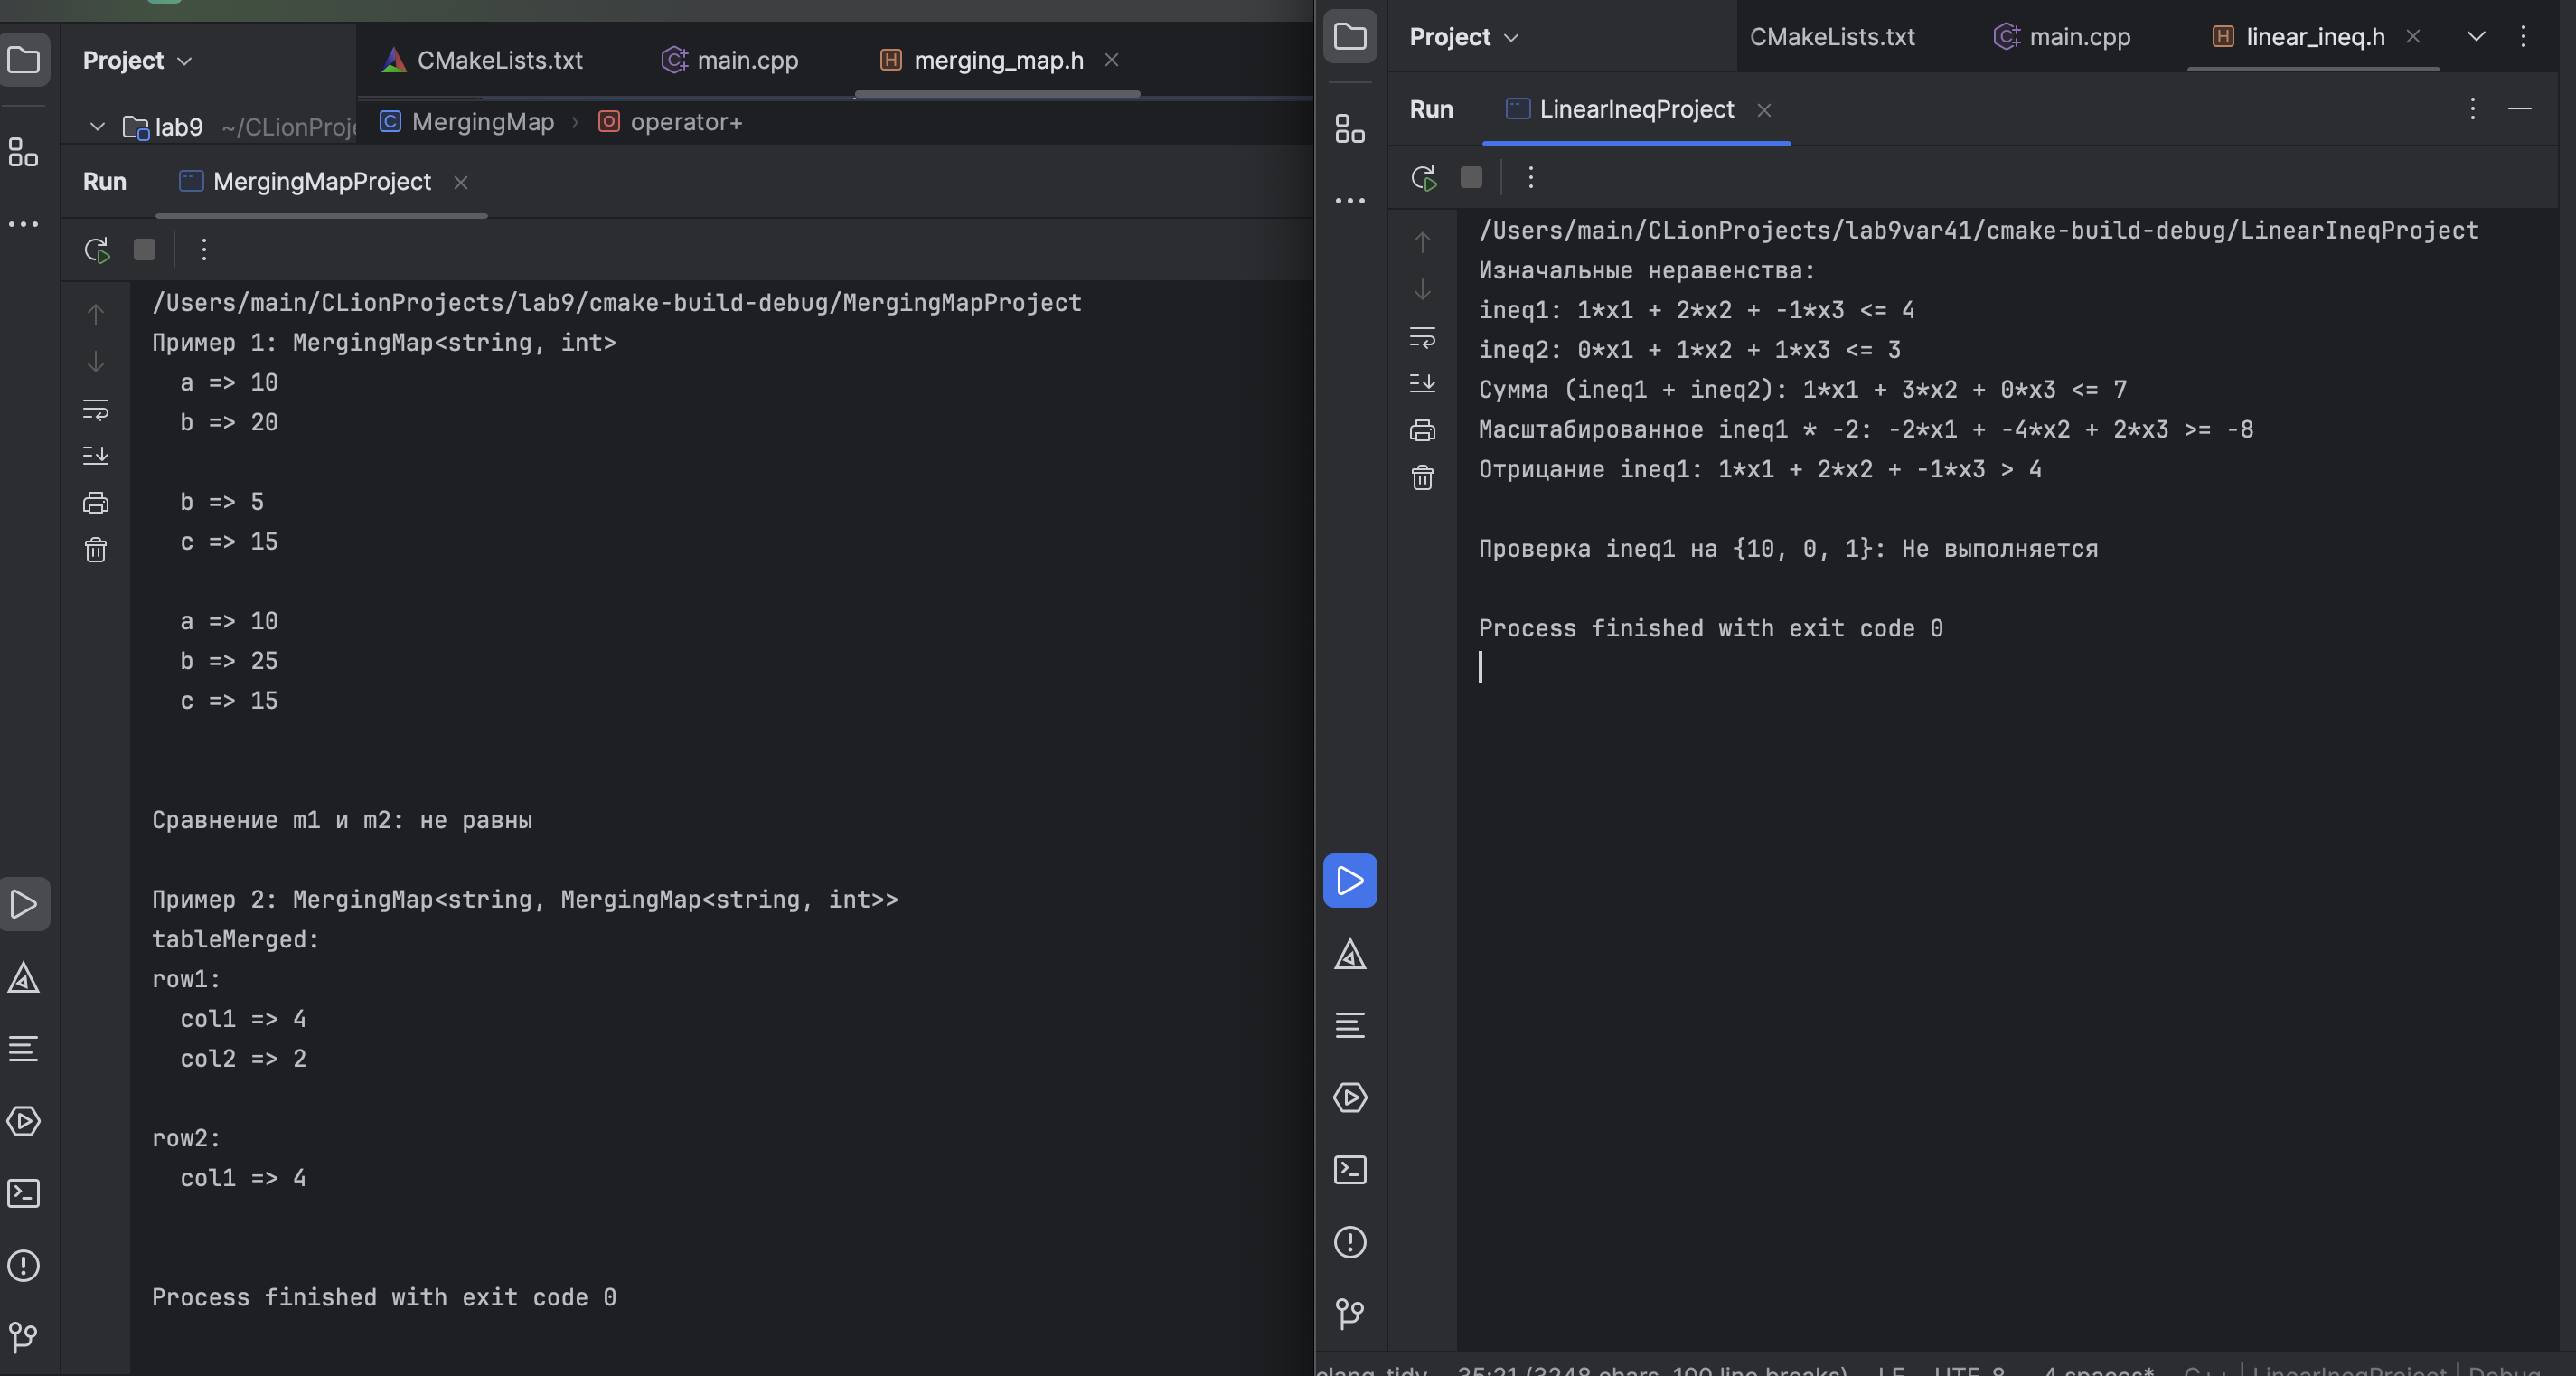
\includegraphics[width=0.8\textwidth]{фото22.jpeg}
  \captionof{figure}{Фрагмент консольного вывода тестовых сценариев}
\end{center}

%--------------------------------------
\section{Вывод}
В лабораторной работе разработаны два обобщённых класса с перегрузкой
операций:

\begin{itemize}[nosep]
  \item \textbf{LinearIneq<T,N>} реализует алгебру линейных неравенств,
        обеспечивая масштабирование, отрицание, сложение и проверку
        истинности для произвольного вектора переменных.
  \item \textbf{MergingMap<K,V>} расширяет стандартное понятие
        ассоциативного массива операцией «слияния», аддитивно объединяя
        значения по совпадающим ключам. Реализована автоматическая
        инициализация «нулём» и сравнение карт.
\end{itemize}

Тестирование на комбинациях примитивных и вложенных типов подтвердило
корректность перегруженных операторов и универсальность шаблонов.
Полученные навыки демонстрируют возможности C++ по созданию
пользовательских контейнеров и домен-специфичных алгебраических структур.
\end{document}
